\chapter{Background}
\label{cha:background}
\graphicspath{ {./resources/} }

\section{Lip Reading}
\label{sec: Lip Reading}
% Intro to what it is
Lip reading is a crucial means of communication. It is one of the few mediums of communication available for people who are hard of hearing or deaf, but all people employ lip reading to a degree. The ability to process the shape of the mouth and lips is essential to everyone during speech processing \cite{lip_reading_used_by_everyone}.\\
Lip reading, or speechreading, refers to being able to understand what a person is saying by using only the visual movements of the face. It is a multimodal communication method; lip reading requires information including the shape of the lips, movement of the tongue and position of the teeth \cite{lip_reading_multimodal}. Context is also crucial for lip reading, having been shown to have a huge impact on the ability to recognise different words \cite{Effects-of-context-type-on-lipreading}.\\
In communication, there are various methods to break down and categorise spoken language. The most popular would likely be \gls{phoneme}s: the fundamental and distinct sounds that are made during speech.
\Gls{viseme}s are another fundamental unit of language. \Gls{viseme}s represent the visual counterparts to \gls{phoneme}s. They are the speech sounds that form similar lip shapes and are thus paramount for lip reading.\\ 
\begin{figure}
\centering
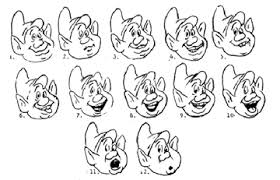
\includegraphics[width=0.5\textwidth]{disney_visemes.jpg}
\caption[The twelve classic Disney \gls{viseme}s.]{The twelve classic Disney \gls{viseme}s. These show the different lip shapes, used by Disney for the 1937 film, Snow White and the Seven Dwarfs, to express different voice noises. Image source: \url{https://docs.cryengine.com/display/SDKDOC2/Phonemes+and+Visemes}}
\label{fig:disney visemes}
\end{figure}
\begin{figure}
\centering
\includegraphics[width=0.5\textwidth]{other_visemes.png}
\caption[OneClick's DAZ Gen8.1 \gls{viseme} example]{OneClick's DAZ Gen8.1. viseme example. These show a more modern, three-dimensional representation of the different \gls{viseme}s used for animation. Image source: \url{https://crazyminnowstudio.com/docs/salsa-lip-sync/modules/recommendations/}}
\label{fig:other visemes}
\end{figure}
However, here is our first problem with lip reading: we do not have a set of consistent \gls{viseme}s. This is primarily an issue highlighted within the domain of animation; animators have to create realistic facial expressions depending on the words being spoken. In the early days of animation, animators realised that different \gls{phoneme}s shared the same facial expression and, therefore, reduced the number of different faces they had to animate. One of the most notable \gls{viseme} sets was Disney's, as shown in Figure~\ref{fig:disney visemes}, which categorises mouth positions into just twelve parts. There are typically ten to fourteen different \gls{viseme}s but there is no global \gls{viseme} set. As shown in Figure~\ref{fig:other visemes}, different animators had different sets of \gls{viseme}s.\\
\begin{figure}
\centering
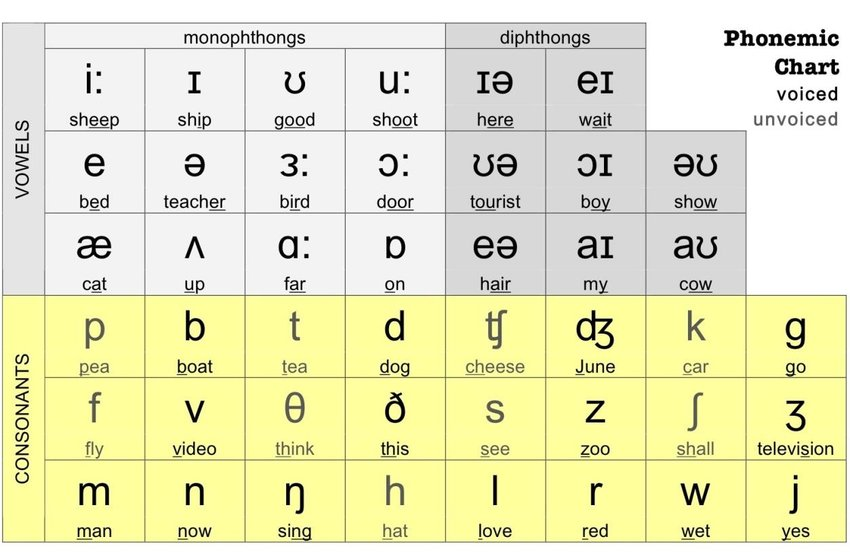
\includegraphics[width=0.5\textwidth]{phoneme_table.png}
\caption[The 44 \Gls{phoneme}s of the English Language.]{The 44 \Gls{phoneme}s of the English Language \cite{44_phonemes}. This represents the widely accepted set of English \gls{phoneme}s, as first presented by Underhil in 2008.}
\label{fig:phoneme table}
\end{figure}
There is another glaring issue with \gls{viseme}s and so lip reading, one that is similar to the everyday homophone. The various \gls{viseme} sets almost always have fewer categories than \gls{phoneme}s do. The consensus in English is that there are 44 unique phonetic sounds, presented in Figure~\ref{fig:phoneme table}. This number is far larger than any set of \gls{viseme}s, which highlights the second major issue with lip reading: the correspondence between \gls{phoneme}s and \gls{viseme}s is tenuous. This is because of visual homophones or homophenes: words that when spoken have different audio components but the same visual components. One of the most famous, and humorous, examples of this is the phrase ``I love you" and ``elephant juice". When spoken aloud these phrases are as different as can be but, for a lip reader, context is needed to tell them apart. Therefore, lip reading is made more complex by the difficult synchronisation between what is spoken and what is visualised.\\
Some studies, such as Bear's ``Which \gls{phoneme}-to-\gls{viseme} maps best improve visual-only computer lip-reading?", have examined which \gls{viseme} sets best map to the \gls{phoneme}s \cite{phoneme_viseme_mapping_review}. However, this study only analyses English \gls{phoneme}s and \gls{viseme}s. As of the time of conducting this research there are 7000 languages spoken worldwide \cite{7000_languages_globally} which might require their own set of \gls{phoneme}s and \gls{viseme}s. There do exist metaphonemes, which are cross-language \gls{phoneme}s \cite{Cross-Linguistic-Phoneme-Correspondences}. However, this would require further analysis into the mapping between these and \gls{viseme}s.\\
Lip reading suffers from all of the difficulties present within classical \acrlong{nlp}, such as homophones, the context being lost, variation in language and ambiguity.\\
Overall, lip reading is an immensely challenging task, one which many fluent speakers can struggle with. From a lack of understanding surrounding \gls{viseme}s, to the thousands of languages spoken around the world, lip reading is hard for people, let alone computers.
\section{Technologies}
This section will delve into the different technologies involved in this research. Various decisions were made surrounding the different tools to employ for data generation, producing a working lip reading model and designing a GUI to showcase the lip reading model.
\subsection{Keras, TensorFlow and PyTorch}
To train \acrshort{ml} models there are two primary libraries: TensorFlow\footnote{\url{https://www.tensorflow.org/}} and PyTorch\footnote{\url{https://pytorch.org/}}. These provide various functionality, such as being able to define \acrlong{anns}, perform mathematical operations on batched data and format sparse or big data. It is important to note that TensorFlow contains another API called Keras\footnote{\url{https://keras.io/}}.\\
There is wide discourse as to which tool is the best. PyTorch is low level, high-performance, easier to debug but less readable. TensorFlow is high and low-level, high-performance, has better readability but is harder to debug. Keras is the most popular of all three. Whilst PyTorch is written in Lua and TensorFlow in a combination of C\texttt{++}, CUDA and Python, Keras is only written in Python. Keras has lower performance but makes up for this with its simplicity and code readability \cite{Keras-vs-TF-vs-PT}. Typically, TensorFlow is regarded as being used more in industry whilst PyTorch is used primarily for research.\\
I decided to go with the popular consensus and use Keras. Its simplicity and readability would be advantageous since I have not made use of any of these tools before. Furthermore, as I am more experienced in Python, this would better suit my skill set. Although it is lower performance than the other libraries, I will only be creating relatively small models and have access to quite powerful \acrshort{gpu}s for training. Furthermore, this research may be useful to get more experience in the industry standard libraries employed for \acrshort{ml}.
\subsection{MediaPipe and Dlib}
\label{sec:mediapipe}
\begin{figure}
\centering
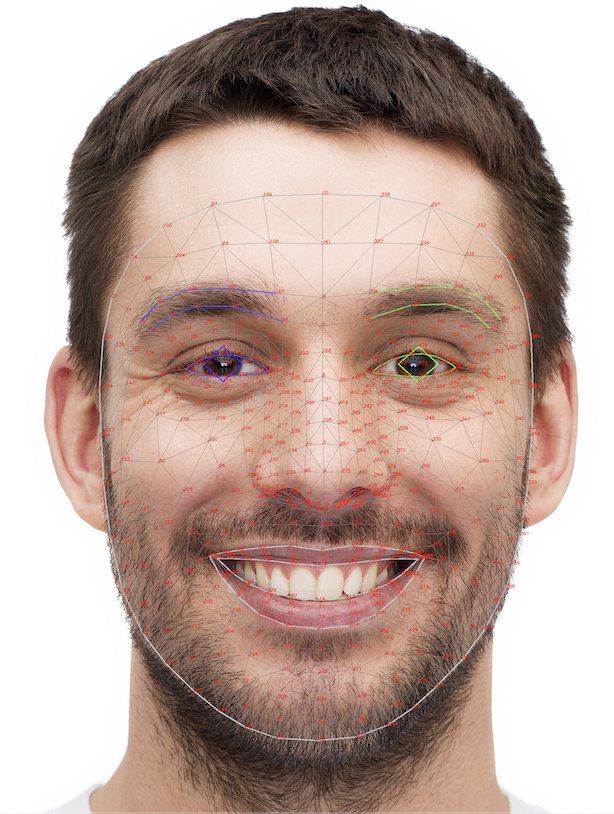
\includegraphics[width=0.5\textwidth]{mediapip_landmarks.png}
\caption[Visualizing the 478 MediaPipe facial landmark coordinates.]{Visualizing the 478 MediaPipe facial landmark coordinates. This image gives a map of the different MediaPipe facial landmarks, labelling each with its index. Image source: \url{https://developers.google.com/mediapipe/solutions/vision/face_landmarker}}
\label{fig:mediapipe landmarks}
\end{figure}
MediaPipe\footnote{\url{https://developers.google.com/mediapipe}}  is an innovative Machine Learning framework developed by Google. MediaPipe provides various functionalities such as gesture tracking, object classification, audio processing and natural language processing. The framework allows for efficient resource management, allowing both GPU and CPU utilisation to increase the performance of running \acrshort{ml} models \cite{mediapipe_info}. Shown in Figure~\ref{fig:mediapipe landmarks}, one notable tool is MediaPipe's Face Landmark Detection\footnote{\url{https://mediapipe-studio.webapps.google.com/demo/face_landmarker}}. This provides a library for detecting faces within images and estimating hundreds of facial landmarks such as the lips, eyes and nose. \\
\begin{figure}
\centering
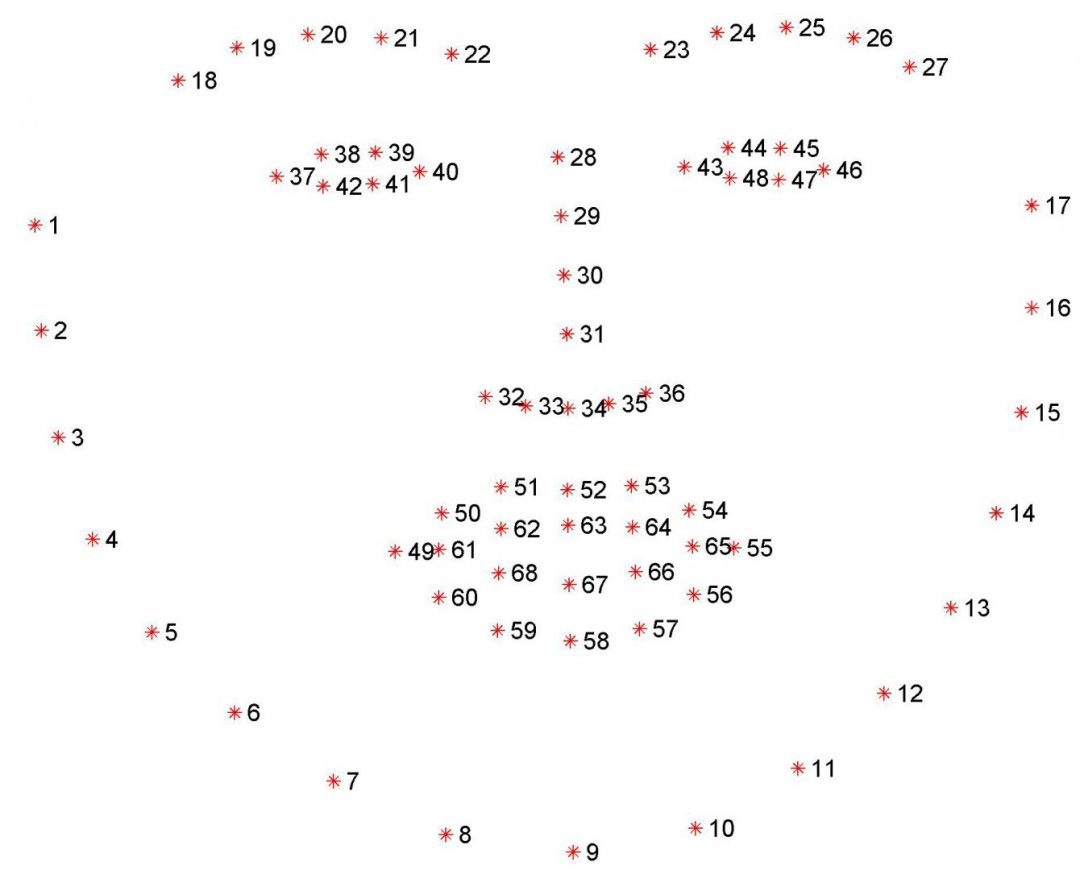
\includegraphics[width=0.5\textwidth]{dlib_landmarks.jpg}
\caption[Visualizing the sixty-eight Dlib facial landmark coordinates.]{Visualizing the sixty-eight Dlib facial landmark coordinates. This gives a map of Dlib's facial landmarks, giving the index of each different landmark. Image source: \url{https://pyimagesearch.com/2017/04/03/facial-landmarks-dlib-opencv-python/}}
\label{fig:dlib landmarks}
\end{figure}
Dlib is a C++ toolkit that contains a diverse selection of Machine Learning solutions. Dlib is primarily a collection of various software components \cite{dlib_info}, the most notable being its Face Detector\footnote{\url{http://dlib.net/face_detector.py.html}}, shown in Figure~\ref{fig:dlib landmarks}. This class can detect faces within images and return the coordinates of facial landmarks.\\
Another major technological decision was whether to utilise MediaPipe or Dlib for collecting data to train the lip reading models. A crucial step for this research is being able to localise to a person's lips to collect data for inference, much like a person does in conversation.\\
In total MediaPipe detects 478 3D facial landmarks, forty of which are directly associated with the lips. Dlib detects sixty-eight 2D facial landmarks, nineteen of which are related to the lips. Further investigation could be done into which performs the best at localising to faces but this difference will likely be insignificant. The more important difference between these two libraries is their landmark data.\\
A major part of \acrshort{ml} is \gls{feature_extraction}. Facial landmarks extracted from images could be useful to train an \acrshort{ann} to focus directly on the shape of the lips when different \gls{phoneme}s are being said. These could significantly cut down on noise within data, using transfer learning to make a more accurate model.\\
Consequently, the clear choice is to use MediaPipe. It provides more information associated with the lips: there are more than double the landmarks, all of which are a higher dimension than the landmarks generated by Dlib.
\subsection{Tkinter}
Tkinter\footnote{\url{https://docs.python.org/3/library/tkinter.html}} is a Python package that interfaces the Tk \acrfull{gui} toolkit. It is a package for producing various cross-platform GUI applications with a native look and feel \cite{An-introduction-to-tkinter}.\\
There is much discussion about which Python GUI package to use, some popular choices include PySimpleGUI\footnote{\url{https://www.pysimplegui.org/en/latest/}}, Flexx\footnote{\url{https://flexx.readthedocs.io/en/stable/}} and Ipywidgets\footnote{\url{https://ipywidgets.readthedocs.io/en/stable/}}.\\
For this project, Tkinter will be used due to its simplicity, ability to be run on different Operating Systems and its accessibility (Tkinter is pre-installed on Python) \cite{comparing_python_guis}. Tkinter has good flexibility and I have experience with this tool already. Therefore, the focus of the project will remain on lip reading rather than learning a new Python \acrshort{gui} tool.
\subsection{NLTK}
\label{sec: nltk}
% For getting phonemes
% Reference here how we get visemes
NLTK\footnote{\url{https://www.nltk.org/}} is a Python library for \acrlong{nlp} and text analytics \cite{nltk_info}. It provides various tools for processing text like lemmatisation, tagging, tokenisation and word normalisation. Moreover, NLTK contains numerous \gls{corpora}.\\
One useful tool provided by NLTK is the Carnegie Mellon Pronouncing Dictionary (cmudict)\footnote{\url{https://www.nltk.org/_modules/nltk/corpus/reader/cmudict.html}}. This reduces English words to their constituent \gls{phoneme}s.\\
As there is no standard set of \gls{viseme}s, NLTK cannot be used as a \acrfull{p2v} mapper: a tool that would be crucial for generating \gls{viseme} data. Research suggests \cite{phoneme_viseme_mapping_review} that the best correspondence between \gls{phoneme}s and \gls{viseme}s is Lee \cite{best_phoneme_viseme_mapping}. This maps \gls{phoneme}s to six consonant \gls{viseme}s and seven vowels \gls{viseme}s. It also has a silence \gls{viseme} \cite{best_phoneme_viseme_mapping}. This \acrshort{p2v} map will be hardcoded into a dictionary to easily convert from \gls{phoneme}s to \gls{viseme}s. So, NLTK could be used to convert words to their constituent \gls{phoneme}s before this \acrshort{p2v} mapping is used to convert again to \gls{viseme}s.
\subsection{JiWER}
\label{sec: JiWER}
JiWER\footnote{\url{https://pypi.org/project/jiwer/}} is a Python library that supports various \acrfull{asr} tasks. JiWER has been used to compare the performance of various \acrshort{asr} systems \cite{jiwer_example}. It provides various useful functions such as calculating the \acrfull{wer} and \acrfull{cer}, intrinsic for comparing lip reading model performance.\\
The \acrshort{wer} is defined as 
\[WER = \frac{S_w + D_w + I_w}{H_w + S_w + D_w} = \frac{S_w + D_w + I_w}{N_w},\]
where $WER$ is the word error rate, $S_w$ the number of substitutions (in the predicted phrase), $D_w$ the number of deletions, $I_w$ the number of insertions, $H_w$ the number of correct words (or hits in the predicted phrase) and $N_w$ is the number of words (in the reference phrase) \cite{jiwer_example}.\\
The \acrshort{cer} is defined similarly, although rather than looking at words it focuses on individual letters
\[CER = \frac{S_c + D_c + I_c}{H_c + S_c + D_c} = \frac{S_c + D_c + I_c}{N_c}.\]
In these equations, the subscript $w$ signifies variables at the word level and subscript $c$ at the character level.
\section{Artificial Neural Networks}
An \acrfull{ann} is a structure inspired by the brain. It is a set of connected artificial nodes, like mathematical functions, that take input from previous nodes and pass this to later nodes.\\
This section will cover various fundamental concepts for \acrshort{ml} and training an \acrshort{ann}.
\subsection{Softmax}
\begin{figure}
\centering
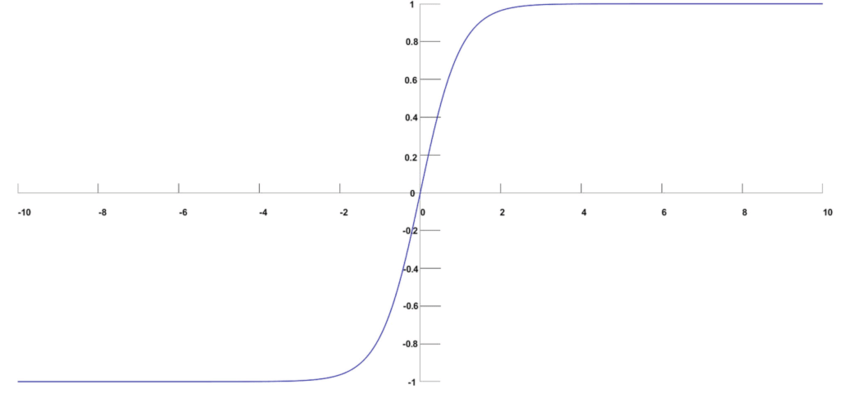
\includegraphics[width=0.7\textwidth]{Softmax-function-image.png}
\caption[Softmax function image.]{Softmax function image \cite{softmax_diagram}.}
\label{fig:softmax}
\end{figure}
Softmax is a crucial but easy mathematical function, shown in Figure~\ref{fig:softmax}, often used as the final \gls{activation_function} within \acrshort{anns}. Softmax is used to normalise a set of numbers so that they sum to 1 \cite{softmax}. Consequently, it is often used to normalise the output of an \acrshort{ann} to give the probability that data samples belong to each class within a set.\\
The Softmax, $\sigma(x)_i$, for each element $x_i$ of a vector is defined as
\[\sigma(\mathbf{x})_i = \frac{e^{x_i}}{\sum^{K}_{j=1}e^{x_j}},\]\\
where there are $K$ classes, $i, j = 1,2,...K$ and $\mathbf{x} = (x_1, x_2,...x_K)$.
\subsection{ReLU}
\label{sec: relu}
\begin{figure}
\centering
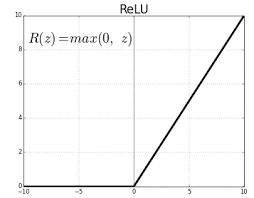
\includegraphics[width=0.5\textwidth]{ReLU Diagram.png}
\caption[Graph of ReLu \gls{activation_function}.]{Graph of ReLu \gls{activation_function}~\cite{relu_diagram}.}
\label{fig:ReLU}
\end{figure}
To train an \acrshort{ann}, the outputs of each layer are passed through a nonlinear function: an \gls{activation_function}. Shown in Figure~\ref{fig:ReLU}, ReLU is a commonly used, simple and efficient \gls{activation_function} within \acrshort{ml} \cite{relu_description}.\\
\acrshort{anns} trained using ReLU typically perform better than those trained using other \gls{activation_function}s, such as the tanh function \cite{relu_is_the_best}.\\
ReLU, $R$, will output the input, $z$ if it is positive but otherwise give the value 0.
\subsection{Cross-Entropy Loss}
\label{sec: Cross-Entropy Loss}
Loss is a crucial measurement within \acrshort{ml}. Loss measures the difference between the predicted and the true classes of data samples. Most methods for training an \acrshort{ann}, such as \acrfull{sgd}, aim at reducing loss for a set of data samples. But, depending on the task, there are many different loss measurements.\\
Cross-entropy loss is employed during training of \acrshort{ann}s that output the probability that a given data sample belongs to a class. Cross-entropy measures the difference between the true probability and a model's predicted probability. A value of 0 means that the model perfectly predicts the probability \cite{cross_entropy_loss}.\\
There are different flavours of cross-entropy, depending on the task. For example, binary cross-entropy is used when there are only two different classes of data. Categorical cross-entropy is used for \gls{multi-class}.\\
In \gls{multi-class}, an \acrshort{ann} will output the probability that a data sample belongs to each different class. Therefore, categorical cross-entropy is employed to increase this probability for the correct class of a sample and reduce the probability for incorrect classes.\\
Categorical cross-entropy will be employed during training of lip reading models as this is a \gls{multi-class} problem; we have a video containing one of $X$ words (or \gls{phoneme}s, or \gls{viseme}s).\\
The formulation for cross-entropy loss, $L$, over $N$ classes is defined as\\
\[L = - \sum_{i=1}^{N} y_i \log{p_i},\]\\
where $y_i$ is the truth value, of whether a data sample is in class $i$, and $p_i$ is the Softmax probability for the class $i$. For training, there are four classes so this can be expanded further:\\
\[L = - [ y_0 \log{p_0} + y_1 \log{p_1} + y_2 \log{p_2} + y_3 \log{p_3}].\]
\subsection{Long-Short Term Memory}
A \acrlong{rnn} is a type of \acrshort{ann} used in \acrfull{dl} for sequential data such as text, audio and videos. There are different types of \acrshort{rnn} classified by their structure, such as classic \acrshort{rnn}, \acrshort{lstm}, \acrshort{gru}, Attention \acrshort{rnn} and \gls{transformer}s. The choice of \acrshort{rnn} unit largely depends on the task being carried out, for example the \gls{transformer} architecture is primarily used for modern large language models such as  ChatGPT\footnote{\url{https://chat.openai.com/}}.\\
\begin{figure}
\centering
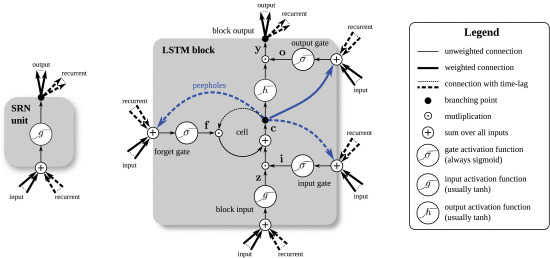
\includegraphics[width=0.9\textwidth]{lstm_diagram.jpg}
\caption[Detailed diagrams of a \acrfull{sru} and \acrfull{lstm} Unit.]{Detailed diagrams of a \acrfull{sru} and \acrfull{lstm} \cite{lstm_diagram}. A \acrshort{sru} is shown on the left and an \acrshort{lstm} block on the right as used in the hidden layers of a recurrent neural network.}
\label{fig:lstm diagram}
\end{figure}
\acrfull{lstm} is an \acrshort{rnn} cell operation first proposed to overcome the vanishing gradient problem \cite{OG_LSTM}. \acrshort{lstm} overcame many of the shortcomings of early, vanilla \acrshort{rnn}s and allowed for both short and longer term dependencies to be established within sequential data.\\
\begin{figure}
\centering
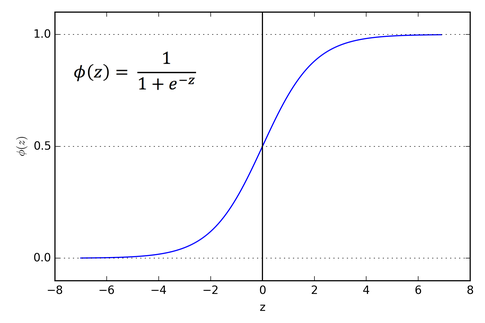
\includegraphics[width=0.5\textwidth]{Sigmoid Activation Function.png}
\caption[Graph of the Sigmoid Activation function.]{Graph of the Sigmoid Activation function. Image source:\\ \url{https://towardsdatascience.com/activation-functions-neural-networks-1cbd9f8d91d6}.}
\label{fig:sigmoid diagram}
\end{figure}
\acrshort{lstm} is comprised of three gates called the input, output and forget gates. Shown in Figure~\ref{fig:lstm diagram}, these gates give \acrshort{lstm}s the ability to alter or drop data from a sequence \cite{Deep-learning:-RNNs-and-LSTM}. This makes them useful for processing video data where there are long-term dependencies between frames and speech containing \gls{speech_disfluency} or features that need to be ignored. The gates are computed using sigmoid \gls{activation_function}s, shown in Figure~\ref{fig:sigmoid diagram}. LSTM has also been shown to be successful for video facial recognition tasks in the past \cite{facial_expression_rec_lstm}.\\
\begin{figure}
\centering
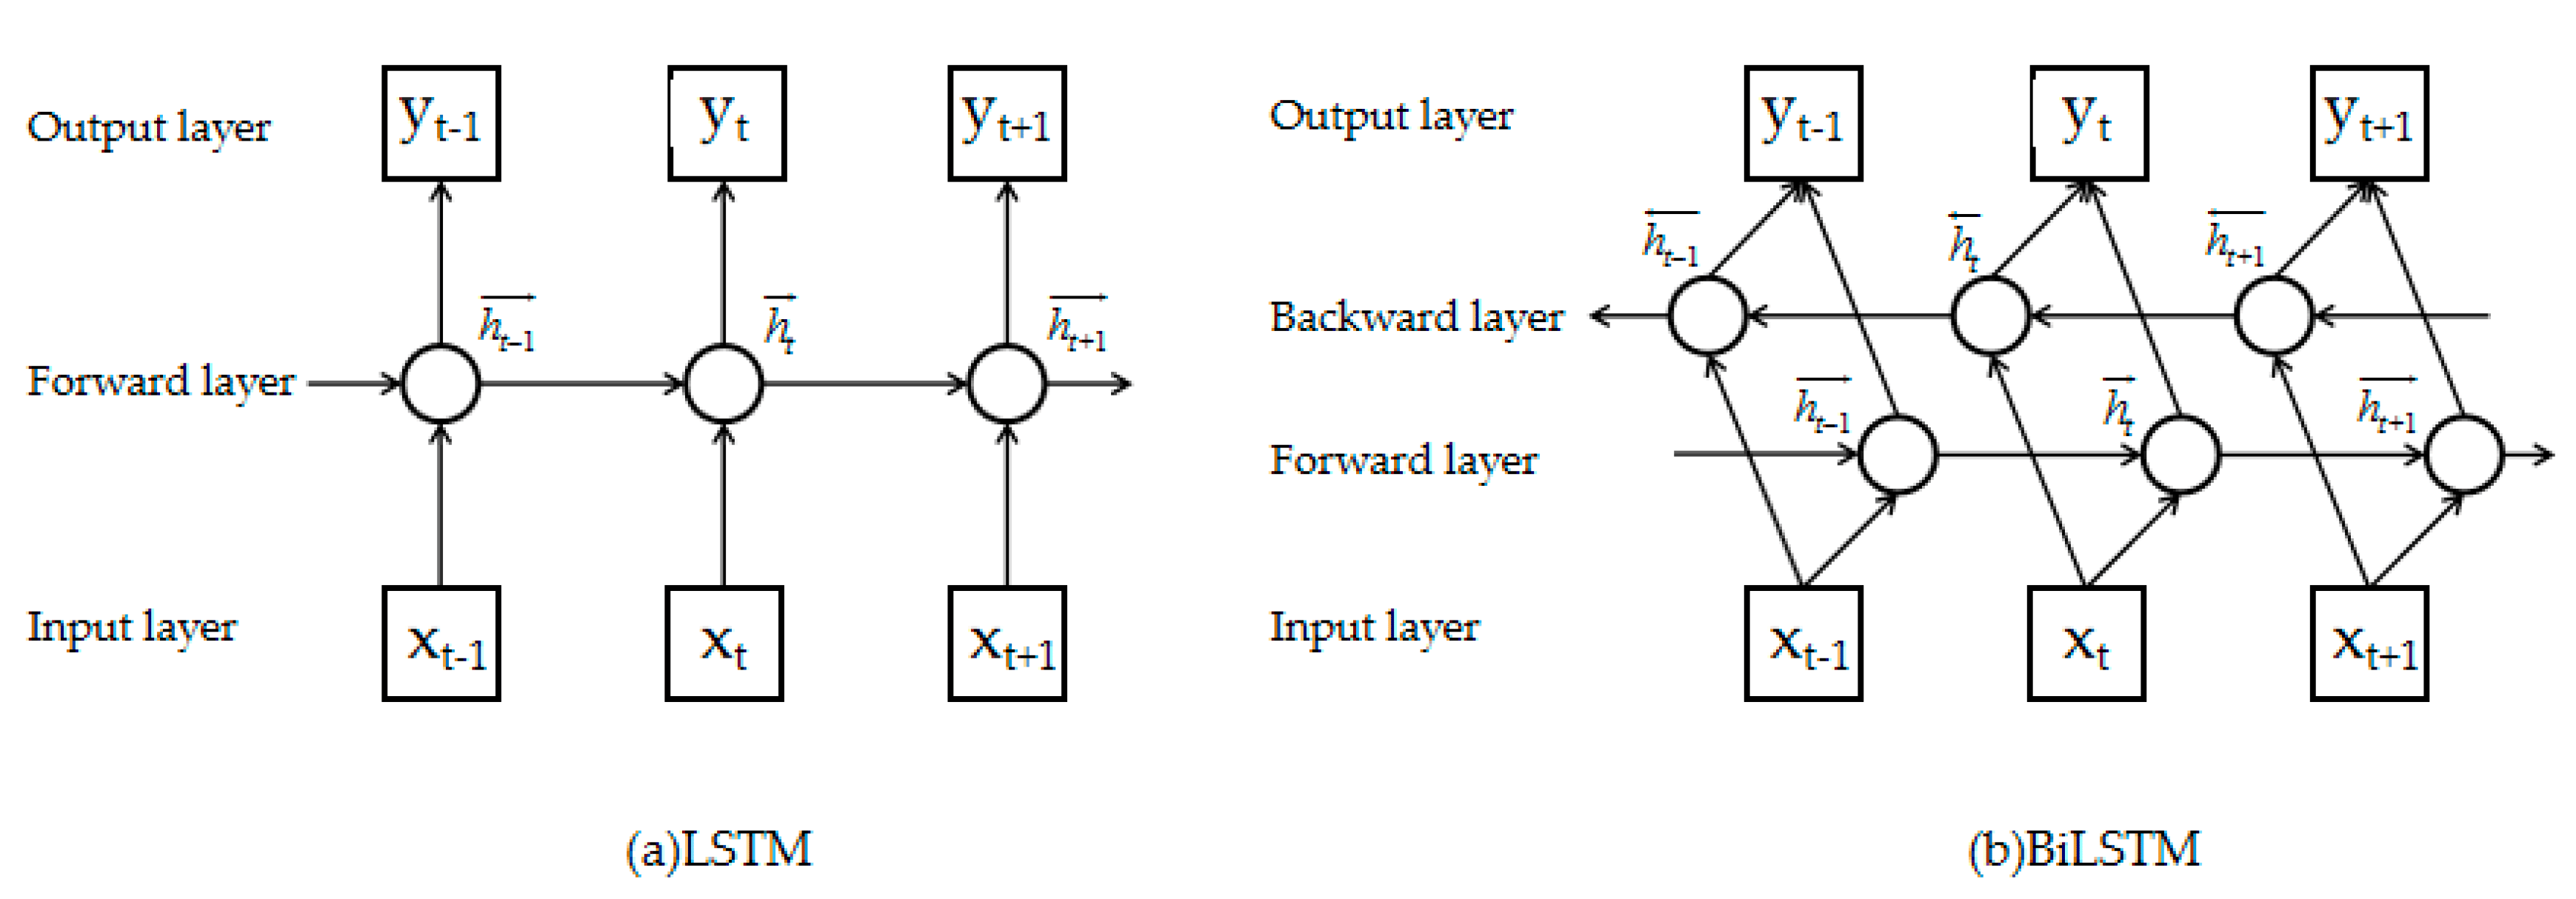
\includegraphics[width=0.7\textwidth]{bilstm.png}
\caption[The architecture of the (a) LSTM model and (b) BiLSTM model.]{The architecture of the (a) LSTM model and (b) BiLSTM model~\cite{bilstm_diagram}.}
\label{fig:bilstm diagram}
\end{figure}
A notable extension to typical \acrshort{rnn}s is that of a bidirectional \acrshort{rnn}. This allows consideration of both left and right context: events that happened in both the past and future. Bidirectional \acrshort{rnn}s have been used to derive \acrfull{bilstm} (shown in Figure~\ref{fig:bilstm diagram}) and \acrfull{bigru}. However, the main downside of these networks is that they require training two separate architectures simultaneously.
\subsection{Convolutional Neural Networks}
\begin{figure}
\centering
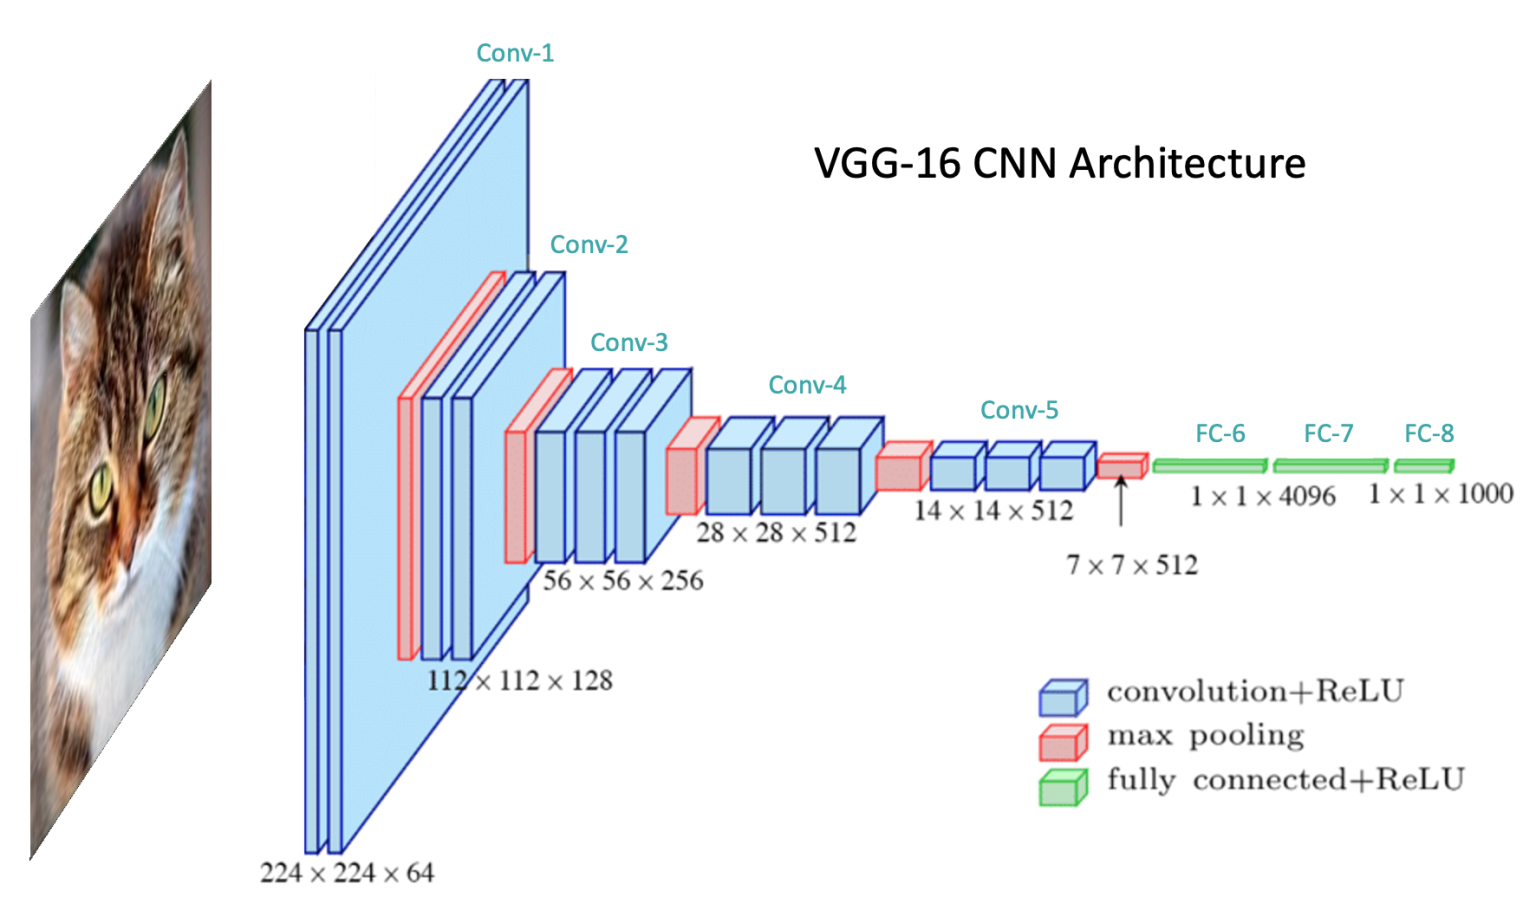
\includegraphics[width=0.7\textwidth]{CNN Diagram.png}
\caption[The VGG-16 \acrfull{cnn} Architecture.]{The VGG-16 \acrfull{cnn} Architecture~\cite{vgg_architecture}. This depicts the main features of a \acrshort{cnn}: convolutional layers, max pooling layers and a final set of fully-connected layers. Image source: \url{https://learnopencv.com/understanding-convolutional-neural-networks-cnn/}}
\label{fig:cnn diagram}
\end{figure}
Primarily used to solve image classification tasks, \acrfull{cnns} are a powerful \acrshort{ann} architecture \cite{cnn_intro, Convolutional-neural-network:-a-review-of...}. \acrshort{cnn}s are characterised by three primary components: convolutional layers, max pooling layers and a final set of fully-connected layers \cite{cnn_intro}.\\
The operation of convolutional layers hinges on filters (also called kernels), comprised of trainable parameters, that are convolved across an image \cite{Convolutional-neural-network-(CNN)-for-image-detection-and-recognition, Convolutional-neural-network:-a-review-of...}. Convolution can be done on images if the layer is the first within the network, like \emph{Conv-1} in Figure~\ref{fig:cnn diagram}, or otherwise the output from the previous layer, called a hidden representation.\\
Convolution functions by the filter being slid across the input array. The scalar product between the filter and the current image region is calculated and placed at the centre point of the filter within the image.\\
The output, $C$, of a convolutional layer at the position $(a,b)$ is thus given as
\[C_{a,b} = \sum^{f-1}_{i=0}\sum^{f-1}_{j=0}w_{i,j} \cdot X_{i+a,j+b},\]\\
where $X$ is the input, of size $N\times N$, and $w$ is the filter, of size $f\times f$.\\
Presented here is 2D convolution, however, there also exists 1D and 3D convolutional layers, the difference being the filter and data size. 3D convolution is typically used for video data and requires 3D matrices of filters.\\ 
Max pooling layers are simpler, instead being used to reduce the size of a hidden representation within a model \cite{cnn_intro}. Max pooling layers similarly convolve across the output of the previous \acrshort{ann} layer, taking the maximum value in each pooling region to be the output, thus capturing the strongest activations \cite{max_pooling_&_dropout}. This effectively reduces the effect of noise and reduces the size of data whilst remaining computationally efficient.\\
The output of a max pooling layer, $M$, at the position $(i,j)$ and the size of the output, $m$, are defined as
\[M_{i,j} = max(X_{i-(f/2),j-(f/2)},...X_{i+(f/2),j+(f/2)}),\]
\[m = \frac{N - f}{s} + 1,\]
where $s$ is the stride size: how many positions the filter is moved in each operation \cite{Pooling-methods-in-deep-neural-networks}.\\
A fully-connected layer is classified by its neurons. Every neuron of a fully-connected layer is connected to every single neuron from the previous layer \cite{cnn_intro}.\\
Overall, \acrshort{cnn}s are fantastic to better visualise and identify possible problems models may have with the underlying data thus forming useful, general models to be used for \gls{feature_extraction} or otherwise \cite{Visualizing-and-understanding-convolutional-networks}. \acrshort{cnn}s have proven themselves time and time again as excellent architectures for visual-based models.
\subsection{Attention}
\label{sec: Attention}
Attention is a modern and popular method for speech recognition and language-based problems \cite{Effective-Approaches-to-Attention-based-Neural-Machine-Translation}. It offers fantastic performance for machine translation and is capable of understanding longer utterances than those present within the training data \cite{Attention-based-models-for-speech-recognition}. Some similar work, with attention for lip reading, has even used this to great success in the past \cite{lipreading_with_attention}.\\
Attention mimics how humans form information: by selectively building connections between different parts of information, rather than considering the entire context at once \cite{A-review-on-the-attention-mechanism}. The major benefit of this, for lip reading, is that it allows for ignoring \gls{speech_disfluency}, mapping varying numbers of states within the input sequence to the output sequence and focusing on crucial details within a sequence.\\
To calculate attention, there are three main components: the key ($K$), the query ($Q$), and the value ($V$). $K$ encodes the source data feature, $Q$ is a task-related representation (often the output we want to get) and $V$ is a new data feature representation \cite{A-review-on-the-attention-mechanism}. $V$ is usually an alternate representation of the original sequence or even just the same as $K$ \cite{A-review-on-the-attention-mechanism}.\\ 
Here the standard, scaled dot-product attention will be used, rather than the other forms of attention. This is the default offered by the Keras library\footnote{\url{https://keras.io/api/layers/attention_layers/attention/}}. This is defined as
\[Attention(Q, K, V) = softmax(\frac{QK^{T}}{\sqrt{|K|}}) \cdot V,\]\\
where $Q$ is the query, $K$ is the key and $V$ is the value.\\
Self attention is defined as attention where $Q$, $K$ and $V$ are all the same sequence. This method offers the advantage of self-alignment, enabling the identification of the importance of particular states within a sequence in relation to other states \cite{self_attention}.
\subsection{Stochastic Gradient Descent}
\begin{figure}
\centering
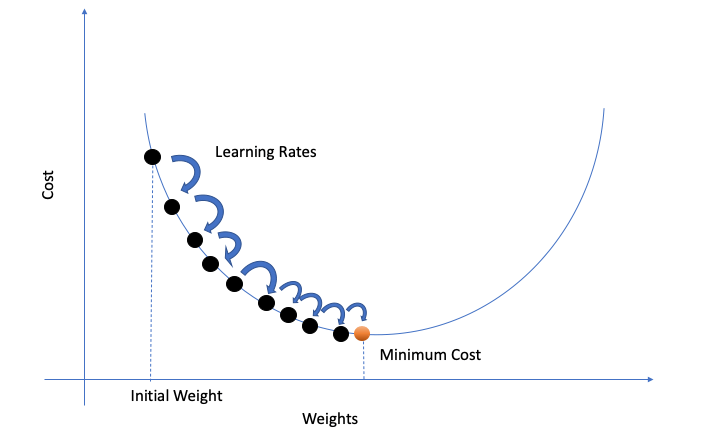
\includegraphics[width=0.7\textwidth]{Stochastic-Gradient-Descent.png}
\caption[Stochastic Gradient Descent.]{Stochastic Gradient Descent~\cite{sgd_diagram}. Here we can see how cost, or loss, is reduced via Stochastic Gradient Descent. This is the ideal for training, where we want to optimise our weights to achieve as small a loss as possible and so an optimal model.}
\label{fig:Stochastic Gradient Descent}
\end{figure}
Training an \acrshort{ann} is an iterative optimisation problem, where the goal is to find the inputs that minimise the output of an objective function \cite{Stochastic-gradient-descent}. At present, gradient descent is the most popular method for solving such a problem. Gradient descent, represented in Figure~\ref{fig:Stochastic Gradient Descent}, uses the first-order derivative to make small, iterative steps in the opposite direction to the gradient of the loss function. This leads to the minima and the most optimal \acrshort{ann} weights for a given problem.\\
Stochastic mini-batch gradient descent is a variation of this process, where each update utilises a random subset of data samples to adjust the network weights \cite{Stochastic-gradient-descent}. This is opposed to just using a single data sample or the entire dataset (stochastic and batch gradient descent, respectively). Mini-batch gradient descent boasts several advantages over other methods, such as reduced computational cost, reduced noise and \gls{overfitting} avoidance \cite{Stochastic-gradient-descent}.\\
Two parameters crucial to \acrshort{sgd} are \acrlong{lr} and batch size.\\
\subsubsection{Learning Rate}
\begin{figure}
\centering
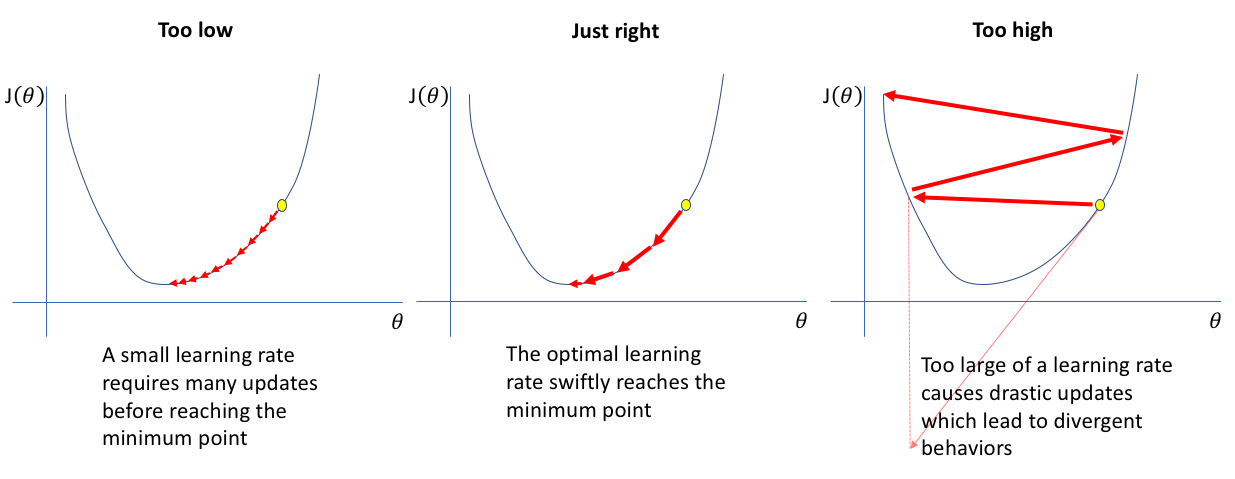
\includegraphics[width=0.7\textwidth]{Learning Rate.png}
\caption[The effects of varying \acrshort{lr}.]{The effects varying \acrshort{lr}. This shows how too high or low \acrshort{lr} can cause problems when minimising a loss function. Image source: \url{https://www.jeremyjordan.me/nn-learning-rate/}.}
\label{fig:Learning Rate}
\end{figure}
\acrfull{lr} relates to the size of steps within \acrshort{sgd}. Finding the optimal \acrshort{lr} is a difficult task requiring tuning \cite{adadelta_adaptive_learning_rate}. As show in Figure~\ref{fig:Learning Rate}, electing too high an \acrshort{lr} could prevent any minima ever being found, whilst too low could slow training significantly and find local minima \cite{adadelta_adaptive_learning_rate}. \acrshort{lr} is one of the leading causes of \gls{overfitting} within \acrshort{ml}, so is a crucial design decision \cite{learning_rate_causes_overfitting}.\\
\begin{figure}
\centering
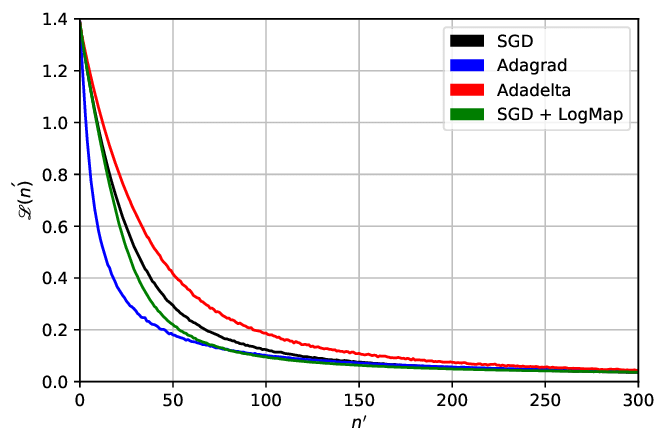
\includegraphics[width=0.7\textwidth]{Adaptive Learning Rate.png}
\caption[The advantage of Adagrad with the adaptive \acrshort{lr} over other \acrshort{lr} methods.]{The advantage of Adagrad with the adaptive \acrshort{lr} over other \acrshort{lr} methods~\cite{adaptive_learning_rate_diagram}. This shows the impact of utilising Adagrad, an adaptive \acrshort{lr} scheduler over regular \acrshort{sgd}. Here the same loss was achieved in far fewer epochs. The choice of \acrshort{lr} scheduler is crucial as it could produce worse results, such as with Adadelta.}
\label{fig:Adaptive Learning Rate}
\end{figure}
Recently multiple methods have been developed to vary \acrshort{lr} over time, rather than keeping it static throughout training \cite{Learning-an-adaptive-learning-rate-schedule}. Some of the different dynamic \acrshort{lr}s are shown in Figure~\ref{fig:Adaptive Learning Rate}. Adaptive \acrshort{lr} can save computational time whilst still finding the global minimum: the best of both stochastic and batch gradient descent.\\
The choice of \acrshort{lr} scheduler, or optimiser, is incredibly important, possibly increasing or decreasing the number of epochs required for training. Some examples include linear decay, Adadelta, Adam and exponential decay \cite{Learning-an-adaptive-learning-rate-schedule}.\\
\subsubsection{Batch Size}
\label{sec: Batch Size}
Batch size is the number of samples used within one training pass of a neural network \cite{batch-size-on-the-generalizability}. Difficult to tune, batch size dramatically impacts the performance of neural networks.\\
Various research has been done into the impact of batch size, concluding that, for image classification, a higher batch size produces better performance \cite{batch-size-on-the-performance}. However, this is not always the case. The option of batch size depends on the task being carried out and the other hyperparameters within the experiment \cite{batch-size-on-the-generalizability}. With a large \acrshort{lr} it is better to use a large batch size, and for a small \acrshort{lr}, a small batch size is better \cite{batch-size-on-the-generalizability}.\\
This is due to the roles of batch size and \acrshort{lr}. With a high \acrshort{lr} we have that the model changes dramatically based on the data but if we have a small batch size and little data, the model may become biased towards just these samples. Models could overfit, becoming too focused on the small dataset given. Alternatively, with a low \acrshort{lr} and high batch size, the model may not learn any new information or change very much.\\
Another side effect of batch size is computational cost and efficiency. Larger batch sizes necessitate more calculations thus incurring increased computational costs \cite{batch-size-on-the-performance}. However, larger batch sizes can increase computational efficiency attributed to better data and operation parallelism \cite{Adaptive-Batch-Sizes}.\\
To optimise the training process, a high \acrshort{lr} and batch size should be used initially, reducing these values throughout until only finetuning is required \cite{batch-size-on-the-generalizability}. This balances computational cost and model efficiency. Suggested values for the batch size are around 32 samples and, therefore, this will be used within the experiments unless a more suitable size is identified.
\subsection{Connectionist Temporal Classification Loss}
\label{sec: CTC Loss}
\begin{figure}
\centering
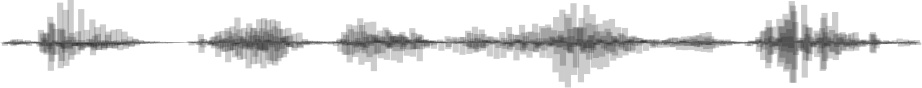
\includegraphics[width=0.7\textwidth]{CTC Audio.png}
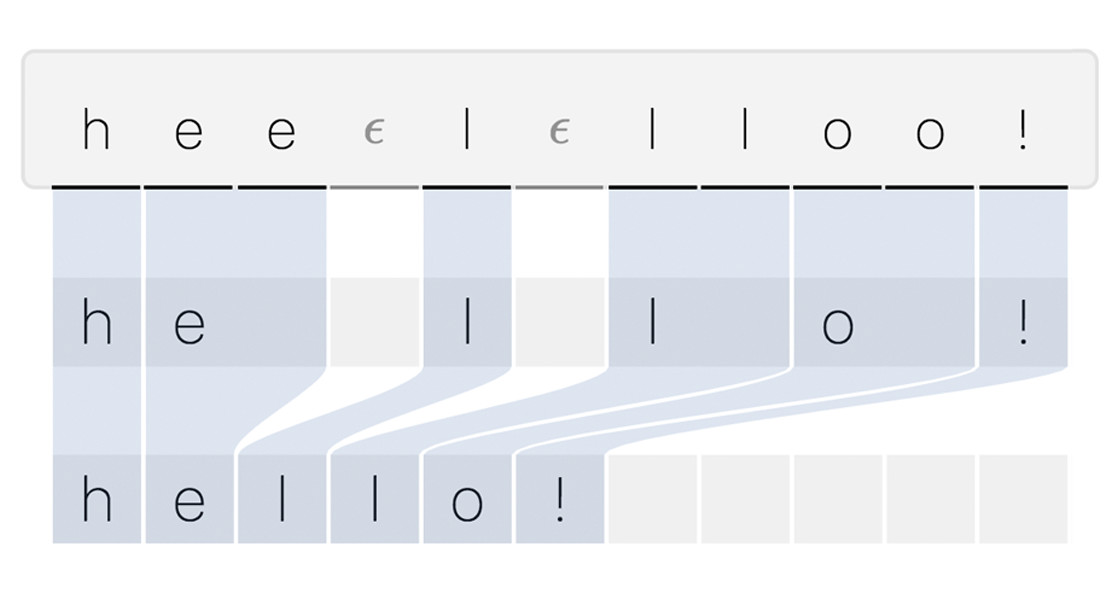
\includegraphics[width=0.7\textwidth]{CTC Loss.jpg}
\caption[\acrshort{ctc} Loss on an audio sequence.]{\acrshort{ctc} Loss on an audio sequence. This shows how CTC loss can be used to predict a sequence of tokens which can then be merged into spoken information. Image source: \url{https://distill.pub/2017/ctc/}.}
\label{fig:CTC Loss}
\end{figure}
\acrfull{ctc} \cite{original_CTC} is a loss metric utilised for sequencing labelling problems where the alignment between the sequence and labels is unknown \cite{exploration-of-CTC-acoustic-models}. The type of alignment found using \acrshort{ctc} loss is depicted within Figure~\ref{fig:CTC Loss}. \acrshort{ctc} loss is used for various speech recognition problems including \acrshort{asr} and lip reading, offering excellent performance \cite{LCANet, LipReading-with-3D-2D-CNN-and-word-CTC-models}.\\
\acrshort{ctc} loss automatically learns connections between sequence frames and labels, removing the need for individual frame labelling \cite{exploration-of-CTC-acoustic-models}. Furthermore, compared with other methods, \acrshort{ctc} loss produces models that are smaller and faster \cite{ctc_faster_models}. Much work has been done within this area and so this method will additionally be incorporated and compared with others for lip reading.\\
For lip reading, \acrshort{ctc} loss will take the form of finding the most likely words (or letters, phonemes or visemes) given the input video feed.\\
First proposed in 2006, \acrshort{ctc} loss aims to find the most likely label sequence, $Y = (y_1, y_2,..., y_U)$ for a given input sequence, $X = (x_1, x_2,...,x_T)$ \cite{original_CTC}. Here, $y(u)$ is the target symbol at time step $u$ and $x(t)$ is the input state at time step $t$. So, we can define the output sequence, $Y^*$ as
\[Y^* = \argmax_Y  P(Y|X)\]\\
This probability is simplified to
\[P(Y|X) = \Sigma_{A \in X, Y} P(A|X)\]
\[P(Y|X) = \Sigma_{A \in X, Y} \prod_{t = 1}^T P_t(a_t|X)\]
\[\therefore Y^* = \argmax_Y \Sigma_{A \in X, Y} \prod_{t = 1}^T P_t(a_t|X)\]\\
Where $A$ represents the alignments from the input to output sequence and $a_t$ the alignment at time step $t$ \cite{original_CTC}.\\
This can then be used to train the model's parameters. By trying to maximise the likelihood of the correct $Y^*$ or minimising the negative log-likelihood  (shown below), we can optimise the model's parameters \cite{original_CTC}.
\[CTC\ Loss = - \Sigma_{(X, Y)} log P(Y|X)\]\\
Training using CTC loss is computationally expensive, as finding the optimal alignments, requires dynamic programming \cite{original_CTC}.
\section{Related Work}
It is important to understand the accomplishments and failures of past work, in the field of automated lip reading, to inform a way forwards.\\
One of the most famous lip reading solutions was proposed by Chung et al.~\cite{Lip-Reading-In-The-Wild} in 2016. Chung et al. generated a huge dataset of word utterances from BBC\footnote{\url{https://www.bbc.co.uk/}} broadcasts, now referred to as \gls{lrw}. This was key to the development of lip reading models and made it possible for others to build upon their work. Their published dataset became widely used due to its easy access and high quality.\\
They proposed a series of different \acrshort{cnn} based architectures for lip reading, which exceeded the public performance benchmark at the time. Furthermore, they speculated about utilising \acrshort{lstm} units to better understand full sentences, rather than just single utterances. This forms a good place to start training.\\
In 2020, Luo et al.~\cite{Synchronous-Bidirectional-Learning-for-Multilingual-Lip-Reading} utilised an encoder and bidirectional decoder architecture to carry out multilingual lip reading by classifying phonemes. This research presented state-of-the-art performance within two benchmarks: English and Mandarin lip reading. Luo et al. proved the usefulness of phonemes, especially across different languages, and the benefit of bi-directional learning.\\  
Just before this work commenced, in 2023 Xue et al.~\cite{lipreading_with_attention} proposed LipFormer, a sequence-to-sequence \gls{transformer} that utilised self and cross attention, \acrshort{gru} units and a combination of visual and landmark features. LipFormer was proposed for the task of visual-only Mandarin Chinese lip reading and could generate both the Pinyin and Chinese characters for a given sequence. This work confirmed that lip landmarks help lip reading and can reduce the \acrfull{wer} of this task~\cite{lipreading_with_attention}.